Esta estructura de datos proporciona las siguientes capacidades. Se nos dan varios elementos, cada uno de los cuales es un conjunto separado. Una DSU tendrá una operación para combinar dos conjuntos y podrá decir en qué conjunto se encuentra un elemento específico. La versión clásica también introduce una tercera operación, puede crear un conjunto a partir de un nuevo elemento.

Por lo tanto, la interfaz básica de esta estructura de datos consta de solo tres operaciones:

\begin{itemize}
	\item \textbf{make\_set(v):} crea un nuevo conjunto que consiste en el nuevo elemento $v$
	\item \textbf{union\_sets(a, b):} fusiona los dos conjuntos especificados (el conjunto en que  se encuentra el elemento $a$ y el conjunto en que se encuentra el elemento $b$)
	\item \textbf{find\_set(v):} devuelve el representante (también llamado líder) del conjunto que contiene el elemento $v$. Este representante es un elemento de su conjunto correspondiente. Se selecciona en cada conjunto por la propia estructura de datos (y puede cambiar con el tiempo, es decir, después de $union\_sets$ las llamadas). Este representante se puede utilizar para comprobar si dos elementos forman parte del mismo conjunto o no. a y b están exactamente en el mismo conjunto, si $find\_set(a) == find\_set(b)$. De lo contrario, están en conjuntos diferentes.
\end{itemize}

Almacenaremos los conjuntos en forma de árboles : cada árbol corresponderá a un conjunto. Y la raíz del árbol será la representante/líder del conjunto.

En la siguiente imagen puedes ver la representación de dichos árboles.

% TODO: \usepackage{graphicx} required
\begin{figure}[h!]
	\centering
	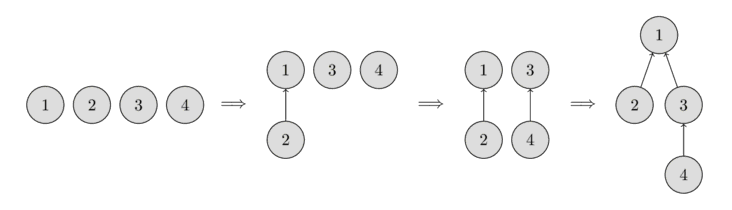
\includegraphics[width=0.7\linewidth]{img/DSU_example}
	\label{fig:dsuexample}
\end{figure}

Al principio, cada elemento comienza como un solo conjunto, por lo tanto, cada vértice es su propio árbol. Luego combinamos el conjunto que contiene el elemento 1 y el conjunto que contiene el elemento 2. Luego combinamos el conjunto que contiene el elemento 3 y el conjunto que contiene el elemento 4. Y en el último paso, combinamos el conjunto que contiene el elemento 1 y el conjunto que contiene el elemento 3.

Para la implementación, esto significa que tendremos que mantener un arreglo $parent$ que almacene una referencia a su ancestro inmediato en el árbol.

\subsection{Implementación sencilla}

La primera implementación de la estructura de datos DSU. Será bastante ineficiente al principio, pero luego podemos mejorarlo usando dos optimizaciones, de modo que tomará un tiempo casi constante para cada llamada de función.

Como decíamos, toda la información sobre los conjuntos de elementos se guardará en un arreglo $parent$.

Para crear un nuevo conjunto (operación $make\_set(v)$), simplemente creamos un árbol con raíz en el vértice $v$, lo que significa que es su propio ancestro.

Para combinar dos conjuntos (operación $union\_sets(a, b)$), primero encontramos el representante del conjunto en el que a se encuentra y el representante del conjunto en el que b se encuentra. Si los representantes son idénticos, que no tenemos nada que hacer, los conjuntos ya están fusionados. De lo contrario, podemos simplemente especificar que uno de los representantes es el padre del otro representante, combinando así los dos árboles.

Finalmente la implementación de la función encontrar representante (operación $find\_set(v)$): simplemente subimos los ancestros del vértice vhasta llegar a la raíz, es decir, un vértice tal que la referencia al ancestro lleva a sí mismo. Esta operación se implementa fácilmente de forma recursiva.

\subsection{Optimización de la compresión de rutas}

Esta optimización está diseñada para acelerar $find\_set$.

Si llamamos $find\_set(v)$ a algún vértice $v$, en realidad encontramos el representante $p$ de todos los vértices que visitamos en el camino entre $v$ y el representante real $p$. El truco consiste en acortar las rutas de todos esos nodos, configurando el padre de cada vértice visitado directamente en $p$.

Puedes ver el funcionamiento en la siguiente imagen. A la izquierda hay un árbol, y a la derecha está el árbol comprimido después de llamar $find\_set(7)$, que acorta los caminos para los nodos visitados 7, 5, 3 y 2.

\begin{figure}[h!]
	\centering
	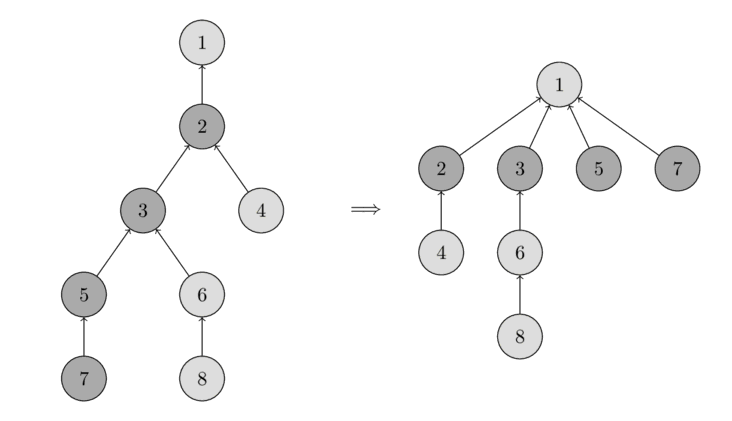
\includegraphics[width=0.6\linewidth]{img/DSU_path_compression}
	\label{fig:dsuexample2}
\end{figure}

\subsection{Unión por tamaño / rango}

En esta optimización cambiaremos la $union\_set$ operación. Para ser precisos, cambiaremos qué árbol se une al otro. En la implementación ingenua, el segundo árbol siempre se adjuntaba al primero. En la práctica, eso puede llevar a que los árboles contengan cadenas de longitud$O(n)$. Con esta optimización evitaremos esto eligiendo con mucho cuidado qué árbol se adjunta.

Hay muchas heurísticas posibles que se pueden utilizar. Los más populares son los siguientes dos enfoques: en el primer enfoque usamos el tamaño de los árboles como rango, y en el segundo usamos la profundidad del árbol (más precisamente, el límite superior de la profundidad del árbol, porque la profundidad se hacen más pequeños al aplicar la compresión de ruta).

En ambos enfoques, la esencia de la optimización es la misma: adjuntamos el árbol con el rango más bajo al que tiene el rango más alto.


